\documentclass{standalone}
\usepackage{tikz}
\usetikzlibrary{patterns, positioning}


\begin{document}
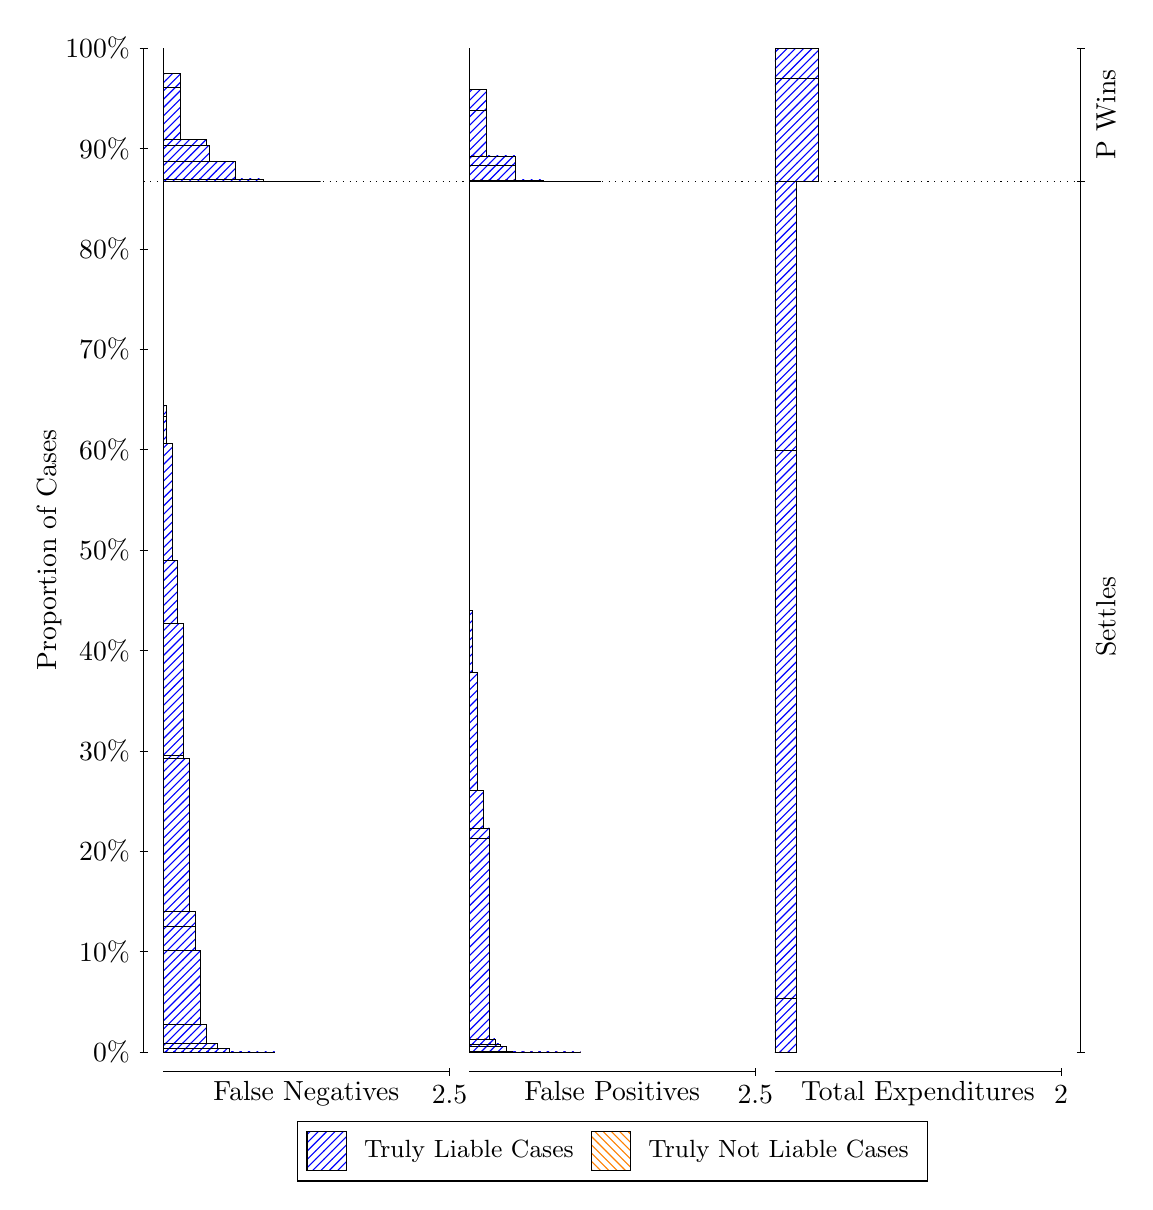
\begin{tikzpicture}
\draw[black, very thin] (1.5,1.75) -- (1.5,14.5);
\node[rotate=90, text=black, anchor=center] at (0.3, 8.125) {Proportion of Cases};
\draw[black, very thin] (1.45,1.75) -- (1.55,1.75);
\node[text=black, anchor=east] at (1.45, 1.75) {0\%};
\draw[black, very thin] (1.45,3.025) -- (1.55,3.025);
\node[text=black, anchor=east] at (1.45, 3.025) {10\%};
\draw[black, very thin] (1.45,4.3) -- (1.55,4.3);
\node[text=black, anchor=east] at (1.45, 4.3) {20\%};
\draw[black, very thin] (1.45,5.575) -- (1.55,5.575);
\node[text=black, anchor=east] at (1.45, 5.575) {30\%};
\draw[black, very thin] (1.45,6.85) -- (1.55,6.85);
\node[text=black, anchor=east] at (1.45, 6.85) {40\%};
\draw[black, very thin] (1.45,8.125) -- (1.55,8.125);
\node[text=black, anchor=east] at (1.45, 8.125) {50\%};
\draw[black, very thin] (1.45,9.4) -- (1.55,9.4);
\node[text=black, anchor=east] at (1.45, 9.4) {60\%};
\draw[black, very thin] (1.45,10.675) -- (1.55,10.675);
\node[text=black, anchor=east] at (1.45, 10.675) {70\%};
\draw[black, very thin] (1.45,11.95) -- (1.55,11.95);
\node[text=black, anchor=east] at (1.45, 11.95) {80\%};
\draw[black, very thin] (1.45,13.225) -- (1.55,13.225);
\node[text=black, anchor=east] at (1.45, 13.225) {90\%};
\draw[black, very thin] (1.45,14.5) -- (1.55,14.5);
\node[text=black, anchor=east] at (1.45, 14.5) {100\%};

\draw[black, very thin] (13.4,1.75) -- (13.4,14.5);
\draw[black, very thin] (13.35,1.75) -- (13.45,1.75);
\node[anchor=west] at (13.35, 1.75) {};
\draw[black, very thin] (13.35,12.806) -- (13.45,12.806);
\node[anchor=west] at (13.35, 12.806) {};
\draw[black, very thin] (13.35,14.5) -- (13.45,14.5);
\node[anchor=west] at (13.35, 14.5) {};

\draw[black, very thin, pattern color=blue, pattern=north east lines] (1.75,1.75) rectangle (3.167,1.75);
\draw[black, very thin, pattern color=blue, pattern=north east lines] (1.75,1.75) rectangle (2.8763,1.75);
\draw[black, very thin, pattern color=blue, pattern=north east lines] (1.75,1.75) rectangle (2.8037,1.75);
\draw[black, very thin, pattern color=blue, pattern=north east lines] (1.75,1.75) rectangle (2.731,1.75);
\draw[black, very thin, pattern color=blue, pattern=north east lines] (1.75,1.75) rectangle (2.5857,1.7953);
\draw[black, very thin, pattern color=blue, pattern=north east lines] (1.75,1.7953) rectangle (2.513,1.7971);
\draw[black, very thin, pattern color=blue, pattern=north east lines] (1.75,1.7971) rectangle (2.4403,1.8616);
\draw[black, very thin, pattern color=blue, pattern=north east lines] (1.75,1.8616) rectangle (2.3677,1.8628);
\draw[black, very thin, pattern color=blue, pattern=north east lines] (1.75,1.8628) rectangle (2.295,2.1041);
\draw[black, very thin, pattern color=blue, pattern=north east lines] (1.75,2.1041) rectangle (2.2223,3.0384);
\draw[black, very thin, pattern color=blue, pattern=north east lines] (1.75,3.0384) rectangle (2.1497,3.3464);
\draw[black, very thin, pattern color=blue, pattern=north east lines] (1.75,3.3464) rectangle (2.1497,3.5398);
\draw[black, very thin, pattern color=blue, pattern=north east lines] (1.75,3.5398) rectangle (2.077,5.4813);
\draw[black, very thin, pattern color=blue, pattern=north east lines] (1.75,5.4813) rectangle (2.0043,5.5131);
\draw[black, very thin, pattern color=blue, pattern=north east lines] (1.75,5.5131) rectangle (2.0043,7.192);
\draw[black, very thin, pattern color=blue, pattern=north east lines] (1.75,7.192) rectangle (1.9317,7.9884);
\draw[black, very thin, pattern color=blue, pattern=north east lines] (1.75,7.9884) rectangle (1.859,9.4829);
\draw[black, very thin, pattern color=blue, pattern=north east lines] (1.75,9.4829) rectangle (1.7863,9.8222);
\draw[black, very thin, pattern color=blue, pattern=north east lines] (1.75,9.8222) rectangle (1.7863,9.9595);
\draw[black, very thin, pattern color=orange, pattern=north west lines] (1.75,9.9595) rectangle (1.75,9.9595);
\draw[black, very thin, pattern color=blue, pattern=north east lines] (1.75,9.9595) rectangle (1.75,12.806);
\draw[black, very thin, pattern color=blue, pattern=north east lines] (1.75,12.806) rectangle (3.7483,12.806);
\draw[black, very thin, pattern color=blue, pattern=north east lines] (1.75,12.806) rectangle (3.385,12.806);
\draw[black, very thin, pattern color=blue, pattern=north east lines] (1.75,12.806) rectangle (3.058,12.806);
\draw[black, very thin, pattern color=blue, pattern=north east lines] (1.75,12.806) rectangle (3.0217,12.839);
\draw[black, very thin, pattern color=blue, pattern=north east lines] (1.75,12.839) rectangle (2.6947,12.839);
\draw[black, very thin, pattern color=blue, pattern=north east lines] (1.75,12.839) rectangle (2.6583,13.063);
\draw[black, very thin, pattern color=blue, pattern=north east lines] (1.75,13.063) rectangle (2.3313,13.262);
\draw[black, very thin, pattern color=blue, pattern=north east lines] (1.75,13.262) rectangle (2.295,13.335);
\draw[black, very thin, pattern color=blue, pattern=north east lines] (1.75,13.335) rectangle (1.968,14.004);
\draw[black, very thin, pattern color=blue, pattern=north east lines] (1.75,14.004) rectangle (1.968,14.177);
\draw[black, very thin, pattern color=blue, pattern=north east lines] (1.75,14.177) rectangle (1.9317,14.177);
\draw[black, very thin, pattern color=orange, pattern=north west lines] (1.75,14.177) rectangle (1.75,14.177);
\draw[black, very thin, pattern color=blue, pattern=north east lines] (1.75,14.177) rectangle (1.75,14.5);
\draw[black, very thin, pattern color=orange, pattern=north west lines] (5.6333,1.75) rectangle (7.0503,1.75);
\draw[black, very thin, pattern color=blue, pattern=north east lines] (5.6333,1.75) rectangle (7.0503,1.75);
\draw[black, very thin, pattern color=orange, pattern=north west lines] (5.6333,1.75) rectangle (6.905,1.75);
\draw[black, very thin, pattern color=blue, pattern=north east lines] (5.6333,1.75) rectangle (6.905,1.75);
\draw[black, very thin, pattern color=orange, pattern=north west lines] (5.6333,1.75) rectangle (6.7597,1.75);
\draw[black, very thin, pattern color=blue, pattern=north east lines] (5.6333,1.75) rectangle (6.7597,1.75);
\draw[black, very thin, pattern color=blue, pattern=north east lines] (5.6333,1.75) rectangle (6.687,1.75);
\draw[black, very thin, pattern color=orange, pattern=north west lines] (5.6333,1.75) rectangle (6.6143,1.75);
\draw[black, very thin, pattern color=blue, pattern=north east lines] (5.6333,1.75) rectangle (6.6143,1.75);
\draw[black, very thin, pattern color=blue, pattern=north east lines] (5.6333,1.75) rectangle (6.5417,1.75);
\draw[black, very thin, pattern color=orange, pattern=north west lines] (5.6333,1.75) rectangle (6.469,1.75);
\draw[black, very thin, pattern color=blue, pattern=north east lines] (5.6333,1.75) rectangle (6.469,1.75);
\draw[black, very thin, pattern color=blue, pattern=north east lines] (5.6333,1.75) rectangle (6.3963,1.75);
\draw[black, very thin, pattern color=orange, pattern=north west lines] (5.6333,1.75) rectangle (6.3237,1.75);
\draw[black, very thin, pattern color=blue, pattern=north east lines] (5.6333,1.75) rectangle (6.3237,1.75);
\draw[black, very thin, pattern color=blue, pattern=north east lines] (5.6333,1.75) rectangle (6.251,1.7503);
\draw[black, very thin, pattern color=orange, pattern=north west lines] (5.6333,1.7503) rectangle (6.1783,1.7503);
\draw[black, very thin, pattern color=blue, pattern=north east lines] (5.6333,1.7503) rectangle (6.1783,1.7546);
\draw[black, very thin, pattern color=blue, pattern=north east lines] (5.6333,1.7546) rectangle (6.1057,1.8185);
\draw[black, very thin, pattern color=blue, pattern=north east lines] (5.6333,1.8185) rectangle (6.033,1.8526);
\draw[black, very thin, pattern color=blue, pattern=north east lines] (5.6333,1.8526) rectangle (5.9603,1.9173);
\draw[black, very thin, pattern color=orange, pattern=north west lines] (5.6333,1.9173) rectangle (5.8877,1.9173);
\draw[black, very thin, pattern color=blue, pattern=north east lines] (5.6333,1.9173) rectangle (5.8877,4.4592);
\draw[black, very thin, pattern color=blue, pattern=north east lines] (5.6333,4.4592) rectangle (5.8877,4.5961);
\draw[black, very thin, pattern color=blue, pattern=north east lines] (5.6333,4.5961) rectangle (5.815,5.0727);
\draw[black, very thin, pattern color=blue, pattern=north east lines] (5.6333,5.0727) rectangle (5.7423,6.5671);
\draw[black, very thin, pattern color=blue, pattern=north east lines] (5.6333,6.5671) rectangle (5.6697,7.3636);
\draw[black, very thin, pattern color=blue, pattern=north east lines] (5.6333,7.3636) rectangle (5.6333,12.806);
\draw[black, very thin, pattern color=orange, pattern=north west lines] (5.6333,12.806) rectangle (7.3047,12.806);
\draw[black, very thin, pattern color=blue, pattern=north east lines] (5.6333,12.806) rectangle (7.3047,12.806);
\draw[black, very thin, pattern color=orange, pattern=north west lines] (5.6333,12.806) rectangle (6.9413,12.806);
\draw[black, very thin, pattern color=blue, pattern=north east lines] (5.6333,12.806) rectangle (6.9413,12.806);
\draw[black, very thin, pattern color=blue, pattern=north east lines] (5.6333,12.806) rectangle (6.9413,12.806);
\draw[black, very thin, pattern color=orange, pattern=north west lines] (5.6333,12.806) rectangle (6.578,12.806);
\draw[black, very thin, pattern color=blue, pattern=north east lines] (5.6333,12.806) rectangle (6.578,12.814);
\draw[black, very thin, pattern color=blue, pattern=north east lines] (5.6333,12.814) rectangle (6.578,12.824);
\draw[black, very thin, pattern color=orange, pattern=north west lines] (5.6333,12.824) rectangle (6.251,12.824);
\draw[black, very thin, pattern color=blue, pattern=north east lines] (5.6333,12.824) rectangle (6.251,12.824);
\draw[black, very thin, pattern color=orange, pattern=north west lines] (5.6333,12.824) rectangle (6.2147,12.824);
\draw[black, very thin, pattern color=blue, pattern=north east lines] (5.6333,12.824) rectangle (6.2147,13.016);
\draw[black, very thin, pattern color=blue, pattern=north east lines] (5.6333,13.016) rectangle (6.2147,13.129);
\draw[black, very thin, pattern color=blue, pattern=north east lines] (5.6333,13.129) rectangle (5.8877,13.129);
\draw[black, very thin, pattern color=orange, pattern=north west lines] (5.6333,13.129) rectangle (5.8877,13.129);
\draw[black, very thin, pattern color=blue, pattern=north east lines] (5.6333,13.129) rectangle (5.8877,13.129);
\draw[black, very thin, pattern color=blue, pattern=north east lines] (5.6333,13.129) rectangle (5.8513,13.712);
\draw[black, very thin, pattern color=blue, pattern=north east lines] (5.6333,13.712) rectangle (5.8513,13.971);
\draw[black, very thin, pattern color=orange, pattern=north west lines] (5.6333,13.971) rectangle (5.6333,13.971);
\draw[black, very thin, pattern color=blue, pattern=north east lines] (5.6333,13.971) rectangle (5.6333,14.5);
\draw[black, very thin, pattern color=orange, pattern=north west lines] (9.5167,1.75) rectangle (9.7892,1.75);
\draw[black, very thin, pattern color=blue, pattern=north east lines] (9.5167,1.75) rectangle (9.7892,2.4376);
\draw[black, very thin, pattern color=orange, pattern=north west lines] (9.5167,2.4376) rectangle (9.7892,2.4376);
\draw[black, very thin, pattern color=blue, pattern=north east lines] (9.5167,2.4376) rectangle (9.7892,9.3856);
\draw[black, very thin, pattern color=orange, pattern=north west lines] (9.5167,9.3856) rectangle (9.7892,9.3856);
\draw[black, very thin, pattern color=blue, pattern=north east lines] (9.5167,9.3856) rectangle (9.7892,12.806);
\draw[black, very thin, pattern color=orange, pattern=north west lines] (9.5167,12.806) rectangle (10.062,12.806);
\draw[black, very thin, pattern color=blue, pattern=north east lines] (9.5167,12.806) rectangle (10.062,14.118);
\draw[black, very thin, pattern color=orange, pattern=north west lines] (9.5167,14.118) rectangle (10.062,14.118);
\draw[black, very thin, pattern color=blue, pattern=north east lines] (9.5167,14.118) rectangle (10.062,14.5);
\draw[black, dotted] (1.5,12.806) -- (13.4,12.806);
\draw[black, very thin] (1.75,1.5) -- (5.3833,1.5);
\node[text=black, anchor=north] at (3.5667, 1.5) {False Negatives};
\draw[black, very thin] (5.3833,1.45) -- (5.3833,1.55);
\node[text=black, anchor=north] at (5.3833, 1.45) {2.5};

\draw[black, very thin] (5.6333,1.5) -- (9.2667,1.5);
\node[text=black, anchor=north] at (7.45, 1.5) {False Positives};
\draw[black, very thin] (9.2667,1.45) -- (9.2667,1.55);
\node[text=black, anchor=north] at (9.2667, 1.45) {2.5};

\draw[black, very thin] (9.5167,1.5) -- (13.15,1.5);
\node[text=black, anchor=north] at (11.333, 1.5) {Total Expenditures};
\draw[black, very thin] (13.15,1.45) -- (13.15,1.55);
\node[text=black, anchor=north] at (13.15, 1.45) {2};

\node[text=black, centered, rotate=90] at (13.72, 7.2778) {Settles};
\node[text=black, centered, rotate=90] at (13.72, 13.653) {P Wins};

\draw (7.449999999999999,1.5) node[draw=none] (baseCoordinate) {};
\begin{scope}[align=center]
        \matrix[scale=0.5, draw=black, below=0.5cm of baseCoordinate, nodes={draw}, column sep=0.1cm]{
            \node[rectangle, draw, minimum width=0.5cm, minimum height=0.5cm, pattern color=blue, pattern=north east lines] {}; &
            \node[draw=none, font=\small, text=black] (B) {Truly Liable Cases}; &
            \node[rectangle, draw, minimum width=0.5cm, minimum height=0.5cm, pattern color=orange, pattern=north west lines] {}; &
            \node[draw=none, font=\small, text=black] (B) {Truly Not Liable Cases}; \\
            };
\end{scope}

\end{tikzpicture}
\end{document}